\graphicspath{{./Aplikacja/images}}

\chapter{Aplikacja pulpitowa}

Aplikacja będąca obiektem tego podrozdziału stanowi rdzeń systemu kontroli, dzięki któremu operator urządzenia jest nim w stanie sterować oraz zbierać z jego pomocą dane. Zawiera ona moduły do komunikacji ze wszystkimi częściami urządzenia oraz zestaw wykresów aktualizowanych w czasie rzeczywistym. Pomimo względnie prostych funkcji, aplikacja posiada złożoną strukturę ze względu na rówoległą obsługę różnych dróg komunikacji. Struktura ta w szczegółach opisana zostanie  w dalszej części tego rozdziału.

\section{Rola i założenia aplikacji}

Aplikacja była rozwijana mając na uwadze poniższe założenia:
\begin{itemize}
	\item Powinna umożliwiać oparatorowi zadanie prędkości obu stopni swobody klinostatu oraz objętości wody, która ma zostać dostarczona co wskazany przez operatora interwał czasowy.
	\item Powinna dawać dostęp do danych o orientacji komory względem wektora grawitacji, uśrednionej grawitacji i temperatury z ostatnich 60 sekund. Dane odnośnie wilgotności podłoża z uwagi na korozję czujnika przeprowadzane są znacznie rzadziej. Dodatkowo na jednym z wykresów przedstawiana ma być transformata Fouriera sygnału uzyskanego z akcelerometru.
	\item Powinna posiadać podstawowe zabezpieczenia, aby uniemożliwić operatorowi zawieszenie urządzenia poprzez nieświadome wykonanie operacji niedozwolonych. Powinny również znaleźć się w niej zabezpieczenia obsługujące błędy generowane przez fizyczne odłączenie klinostatu w momencie gdy program zakłada iż jest on podłączony.
	\item Powinna w tle posiadać uruchomiony moduł komunikacji bezprzewodowej z komorą środowiskową. Połączenie to służyć ma wymianie danych oraz nastawie intensywności oświetlenia.
	\item Oprator powinien mieć możliwość zapisania zebranych wyników pomiarów do pliku .csv.
	\item Powinien istnieć podstawowy system komunikatów, który będzie informować operatora o rezultatach jego operacji.
\end{itemize}

\section{Wybrany język i biblioteki} \label{aplikacja_implementacja}

W celu implementacji aplikacji wybrany został język Python. Wybór ten motywowany był moją dobrą znajomością tego języka oraz poprzednim doświadczeniem w tworzeniu aplikacji z graficznym interfejsem użytkownika w tym języku. Interfejs został stworzony z użyciem biblioteki \textbf{Tkinter}, która oferuje względnie proste tworzenie takich aplikacji w konwencji programowania obiektowego, z której to intensywnie korzystano podczas rozwoju programu. Do realizacji łącza bezprzewodowego z komorą środowiskową wykorzystano bibliotekę \textbf{socket}, pozwalającą na utworzenie takiego łącza w lokalnej sieci poprzez protokół TCP (ang. \angver{Transmission Control Protocl}). Do działania programu niezbędna okazała się biblioteka \textbf{threading}, pozwalająca na współbieżne wykonywanie różnych jego części. Transformacja Fouriera liczona jest 15 razy na sekundę z użyciem biblioteki \textbf{scipy}, a obliczenia te są zrównoleglone za pomocą biblioteki \textbf{multiprocessing} w celu ich przyspieszenia. Wykresy tworzone są wykorzystując popularną bibliotekę \textbf{matplotlib}. Oprócz tego wykorzystano również wiele innych modułów takich jak \textbf{pyserial}, \textbf{yaml}, \textbf{queue} czy \textbf{numpy} w różnych, mniej znaczących celach.

\section{Podział programu na wątki} \label{watki}

Cała aplikacja składa się w jednym momencie z trzech rodzajów wątków:
\begin{itemize}
	\item Wątku głównego - odpowiedzialnego za działanie całej aplikacji oraz tworzenie wykresów.
	\item Wątku serwera TCP - odpowiedzialnego za obsługę przychodzących pakietów danych przez websocket oraz wysyłanie odpowiedzi.
	\item Wątków obsługi portu szeregowego - tworzonych jedynie tymczasowo w momencie gdy należy wysłać i/lub odebrać komendę przez magistralę USB z klinostatem.
\end{itemize}
Docelowo wątek główny miał być odpowiedzialny wyłącznie za uruchamianie innych wątków oraz działanie aplikacji, natomiast tworzenie i akutualizacja wykresów miała być rezultatem działania innego, dodatkowego wątku. Takie rozwiązanie okazało się niemożliwe, ze względu na konstrukcję biblioteki matplotlib, która uniemożliwia tworzenie wykresów przez wątki inne niż główny. Związane jest to z tym iż biblioteka ta nie została stworzona w konwencji \angver{threadsafe} - bezpiecznej w działaniach między wątkami. Przy programowaniu wielowątkowym należy zwracać uwagę na występowanie tzw. wyścigów (ang. \angver{race condition}), które występują w momencie gdy przynajmniej dwa, różne wątki próbują uzyskać dostęp do tej samej, dzielonej zmiennej. Występowanie takich wyścigów jest znane w bibliotece matplotlib, a więc wykorzystywana może być ona wyłącznie w obrębie wątku głównego. Rozwiązaniem problemu wyścigów jest wykorzystanie różnego rodzaju struktur synchronizacyjnych takich jak semafory czy zamki, które zapobiegają ich występowaniu. Z tego rodzaju struktur korzysta również aplikacja.\\

Wątek serwera TCP jest uruchamiany przez użytkownika za pomocą odpowiedniego przycisku. Pozostaje on uruchomiony w tle aż do momentu, w którym operator postanowi zakończyć komunikację. Jego rolą jest odbieranie danych pomiarowych wysłanych z komputera komory środowiskowej oraz odesłanie odpowiedzi zawierającej informacje o obecnie ustawionym poziomie oświetlenia. Ze względu na to iż dane te muszą zostać przekazane do wątku głównego, wymiana ta zachodzi poprzez wykorzystanie struktur \textbf{Queue} z biblioteki \textbf{queue}, które zapobiegają wyścigom pomiędzy wątkami.\\

Ostatnim z wątków występujących w programie jest wątek odpowiedzialny za obsługę portu szeregowego, realizującego komunikację z kontrolerem klinostatu. Jego zadaniem jest uzyskanie dostępu do wcześniej utworzonego połączenia szeregowego, wysłanie pożądanej komendy, a następnie uzyskanie odpowiedzi ze strony klinostatu. Takich wątków w jednej chwili może istnieć kilka, ponieważ w programie zachodzą również zautomatyzowane procesy, które wysyłają komendy do klinostatu. Natomiast dostęp do połączenia w tym samym czasie może uzyskać wyłącznie jeden z nich ze względu na wykorzystanie struktury synchronizacyjnej \textbf{lock}. Powoduje to efektywne kolejkowanie operacji wykonywanych na porcie szeregowym. W przeciwnym wypadku program zwróciłby błąd, gdy połączenie z klinostatem zostałoby otwarte po raz drugi. Schemat struktury wątkowej przedstawiony został na Rys. \ref{fig:watki}.

\begin{figure}
	
	\centering
	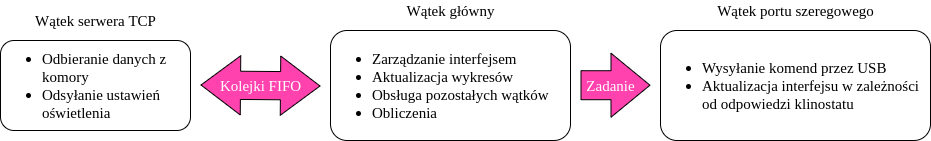
\includegraphics[scale=0.46]{schemat_watki}
	\caption{Schemat budowy wątkowej aplikacji. Źródło: [opracowanie własne]} 
	\label{fig:watki}
	
\end{figure}

\section{Graficzny interfejs użytkownika}

Ten podrozdział poświęcony został opisowemu przedstawieniu graficznego interfejsu użytkownika. Podczas jego tworzenia kierowano się tym, aby był on czytelny, intuicyjny w obsłudze oraz responsywny, aby dawać użytkownikowi pewność iż dokonywane przez niego operacje przynoszą skutek. Interfejs domyślnie po starcie programu jest w znacznej części nieaktywny. Odpowiednie jego sekcje aktywują się gdy pomyślnie zostanie nawiązana komunikacja z kontrolerem klinostatu lub komputerem komory środowiskowej. Taka zmiana uwydatniana jest za poprzez zmianę koloru części interfejsu. Nastawa prędkości klinostatu odbywa się za pomocą dwóch suwaków, które pozwalają na regulację prędkości obu stopni swobody od \SI{0,1}{RPM} do \SI{5}{RPM} z rozdzielczością \SI{0,1}{RPM}. Bezpośrednio obok suwaków znajdują się przyciski odpowiedzialne za uruchomienie bądź zatrzymanie klinostatu. Podgląd tej sekcji interfejsu widoczny jest na Rys. \ref{fig:silniki_gui}. Przyciski oraz ich funkcje, składające się na tę część interfejsu to:
\begin{itemize}
	\item \textbf{Abort} - przycisk natychmiastowo zatrzymujący klinostat bez rampy prędkości. Odpowiada również za wyłączenie hamulców silników gdy klinostat został już wcześniej zatrzymany.
	\item \textbf{Run} - przycisk odpowiedzialny za wysłanie do klinostatu komendy o rozpoczęciu ruchu, oraz przekazaniu mu parametrów prędkości.
	\item \textbf{Pause} - przycisk zatrzymujący klinostat poprzez liniową zmianę prędkości. Po zatrzymaniu, hamulce silników pozostają włączone.
	\item \textbf{Resume} - wznowienie ruchu klinostatu po wcześniejszym zatrzymaniu go poprzez komendę Pause.
	\item \textbf{Echo} - przycisk wysyłający komendę do klinostatu, która wymaga odpowiedzi ze strony jego kontrolera. Jeśli kontroler zwraca jedną z przewidywanych komend, jej skutek wyświetlany jest w aplikacji. Jeśli podczas komunikacji nastąpił błąd, stan całego programu jest resetowany.
\end{itemize}

\begin{figure}
	\centering
	
	\begin{subfigure}[h]{.49\textwidth}
		\centering
			\setlength{\fboxsep}{0pt}
		\setlength{\fboxrule}{1pt}
		\fbox{\includegraphics[scale=1.5]{kontrola_silników}}
		\caption{Nieaktywny interfejs.}
		\label{fig:silniki_gui_nieaktywne}
	\end{subfigure}
	\hfill%
	\begin{subfigure}[h]{.49\textwidth}
		\centering
		\setlength{\fboxsep}{0pt}
		\setlength{\fboxrule}{1pt}
		\fbox{\includegraphics[scale=1.5]{kontrola_silników_aktywny}}
		\caption{Aktywny interfejs.} 
		\label{fig:silniki_gui_aktywne}
	\end{subfigure}
	
	\caption{Interfejs sterowania silnikami. Źródło: [opracowanie własne]}
	\label{fig:silniki_gui}
	
\end{figure}

Sterowanie nawadnianiem odbywa się w podobny sposób. Do dyspozycji są dwa suwaki określające jak często woda ma zostać doprowadzona do środka komory środowiskowej oraz jaka jej objętość za każdym razem będzie do niej trafiać. Na ten blok interfejsu przypadają również trzy przyciski:
\begin{itemize}
	\item \textbf{Start cycle} - rozpoczęcie planu nawadniania według ustawionych parametrów. Jeśli interwał czasowy lub objętość nawadniania zostały ustawiony na wartość zerową, wciśnięcie tego przycisku spowoduje pojawienie się stosownego komunikatu, a cykl się nie rozpocznie.
	\item \textbf{Stop cycle} - przycisk zatrzymujący obecny cykl nawadniania i odblokowywujący ponownie jego nastawę.
	\item \textbf{Force cycle} - przycisk powodujący natychmiastowe wykonanie akcji pompowania o nastawionym parametrze objętościowym. Jeśli w czasie wciśnięcia tego przycisku proces nawadniania trwa, kontroler klinostatu wykryje taką sytuację i zwróci stosowny komunikat do aplikacji.
\end{itemize}
Część interfejsu odpowidzialna za nawadnianie widoczna jest na Rys. \ref{fig:nawadnianie_gui}.\\

\begin{figure}
	\centering
	
	\begin{subfigure}[h]{.49\textwidth}
		\centering
		\setlength{\fboxsep}{0pt}
		\setlength{\fboxrule}{1pt}
		\fbox{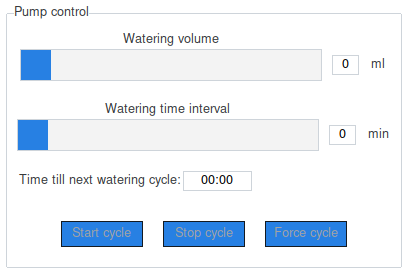
\includegraphics[scale=1.5]{pompa}}
		\caption{Nieaktywny interfejs.}
		\label{fig:woda_gui_nieaktywne}
	\end{subfigure}
	\hfill%
	\begin{subfigure}[h]{.49\textwidth}
		\centering
		\setlength{\fboxsep}{0pt}
		\setlength{\fboxrule}{1pt}
		\fbox{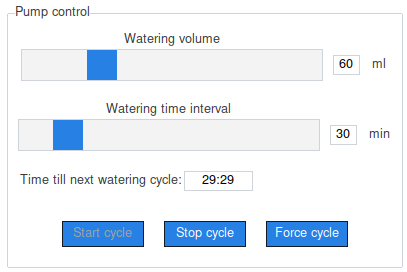
\includegraphics[scale=1.5]{pompa_cykl}}
		\caption{Trwający cykl.} 
		\label{fig:woda_gui_aktywne}
	\end{subfigure}
	
	\caption{Interfejs cyklu nawadniania. Źródło: [opracowanie własne]}
	\label{fig:nawadnianie_gui}
	
\end{figure}\
Kolejnym modułem interfejsu jest kontrola oświetlenia komory środowiskowej widoczna na Rys. \ref{fig:oswietlacz_gui}. W przeciwieństwie do wcześniej opisanych częśći, ten segment pozostaje nieaktywny aż do momentu nawiązania bezprzewodowej komunikacji z komputerem komory klinostatu. Regulacja odbywa się za pomocą określenia intensywności oświetlenia w zakresie od 0 do 100 \%. Wartość ta bezpośrednio odpowiada wypełnieniu sygnału PWM (ang. \angver{Pulse Width Modulation}), którym sterowane są odpowiednie sekcje oświetlenia. Nastawa przekazywana jest przy okazji wymiany informacji z komputerem komory środowiskowej.\\

\begin{figure}[h]
	\centering
	
	\begin{subfigure}[h]{.49\textwidth}
		\centering
		\setlength{\fboxsep}{0pt}
		\setlength{\fboxrule}{1pt}
		\fbox{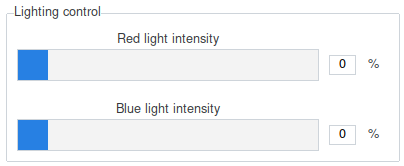
\includegraphics[scale=1.5]{oswietlacz}}
		\caption{Nieaktywny interfejs.}
		\label{fig:oswietlacz_gui_nieaktywne}
	\end{subfigure}
	\hfill%
	\begin{subfigure}[h]{.49\textwidth}
		\centering
		\setlength{\fboxsep}{0pt}
		\setlength{\fboxrule}{1pt}
		\fbox{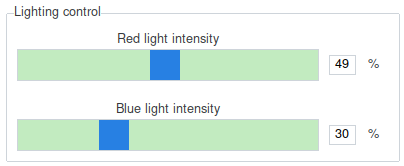
\includegraphics[scale=1.5]{oswietlacz_aktywny}}
		\caption{Aktywny interfejs.} 
		\label{fig:oswietlacz_gui_aktywne}
	\end{subfigure}
	
	\caption{Nastawa oświetlenia. Źródło: [opracowanie własne]}
	\label{fig:oswietlacz_gui}
		
\end{figure}
Jak wspomniano w podrozdziale \ref{aplikacja_implementacja}, połączenie z komputerem komory środowiskowej realizowane jest z użyniem protokołu TCP. Odbywa się to poprzez uruchomienie serwera TCP za pośrednictwem aplikacji przy użyciu przycisku \textbf{Run server}. Jeśli połączenie zostało nawiązane wyświetlony zostanie stosowny komunikat. W przypadku wystąpienia błędu, również zostanie on wyświetlony w wewnętrznej konsoli programu. Aby zerwać połączenie, należy serwer zamknąć naciskając przycisk \textbf{Close server}. Moduł odpowiedzialny za te intrukcje jest widoczny na Rys. \ref{fig:tcp_gui}.\\

\begin{figure}[h]
	
	\centering
	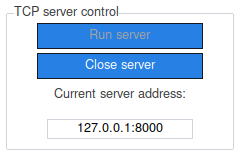
\includegraphics[scale=2]{serwer}
	\caption{Kontrola serwera TCP. Źródło: [opracowanie własne]} 
	\label{fig:tcp_gui}
	
\end{figure}

Bardzo istotnym elementem interfejsu jest konsola w której wyświetlane są komunikaty generowane przez aplikację. Została ona zintegrowana razem z kontrolą połączenia z klinostatem do jednego modułu, przedstawionego na Rys. \ref{fig:konsola_gui}. Na ten moduł składa się rozwijane menu z dostępnymi urządzeniami podłączonymi do portów USB komputera oraz zestaw czterech przycisków:
\begin{itemize}
	\item \textbf{Refresh ports} - przycisk aktualizujący obecnie dostępne urządzenia podłączone do portów szeregowych. Pozwala to wykryć urządzenia, które zostały podłączone do komputera po uruchomieniu aplikacji.
	\item \textbf{Connect} - przycisk inicjujący komunikację z klinostatem przez port USB. Wciśnięcie tego przycisku wysyła komendę do wybranego portu i następnie czeka na odpowiedź. Jeśli otrzymany, powrotny komunikat zgadza się ze spodziewaną komendą klinostatu, interfejs aplikacji zostaje włączony. W konsoli wyświetlany jest stosowny komunikat o błędzie lub pomyślnym połączeniu.
	\item \textbf{Disconnect} - zerwanie połączenia z klinostatem poprze wysłanie odpowiedniej komendy.
	\item \textbf{Clear logs} - przycisk czyszczący komunikaty obecnie znajdujące się w konsoli.
	
\end{itemize}

\begin{figure}[h]
	
	\centering
	\setlength{\fboxsep}{0pt}
	\setlength{\fboxrule}{1pt}
	\fbox{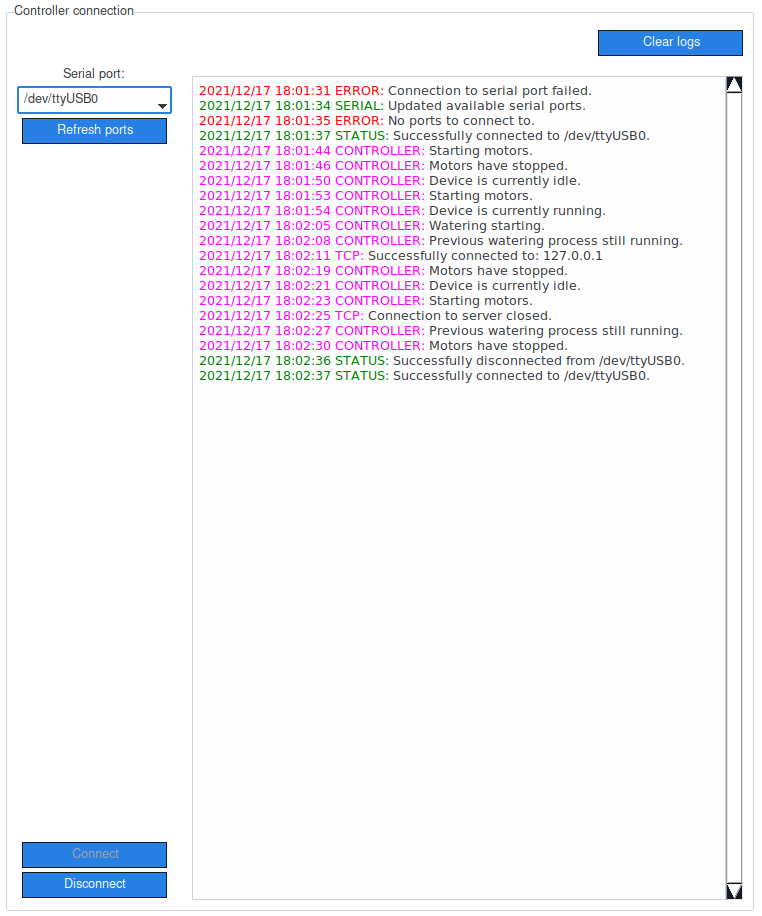
\includegraphics[scale=1.7]{konsola_serial}}
	\caption{Konsola oraz interfejs połączenia szeregowego. Źródło: [opracowanie własne]} 
	\label{fig:konsola_gui}
	
\end{figure}

Cały interfejs podzielony jest na dwie zakładki. Wszystkie dotychczas wymienione elementy znajdują się w zakładce \textit{Clinostat control}. Druga zakładka (\textit{Diagnostics}) zawiera wykresy przedstawiajace zbierane dane w czasie rzeczywistym. Na samym dole zakładni znadjują się dwa przyciski, których zadaniem jest zapisanie lub wyczyszczenie aktualnych danych. Wciśnięcie przycisku \textbf{Save data} spowoduje pojawienie się okna dialogowego w którym należy wybrać ścieżkę oraz nazwę zapisywanego pliku csv. Przycisk \textbf{Clear data} pyta użytkownika czy na pewno chce usunąć zebrane dane, a następnie wykonuje jego wolę. Przykładowe wykresy z rzeczywistymi danymi przedstawione zostały na Rys. \ref{fig:wykresy_gui}.

\begin{figure}[h]
	\centering
	
	\begin{subfigure}[h]{.49\textwidth}
		\centering
		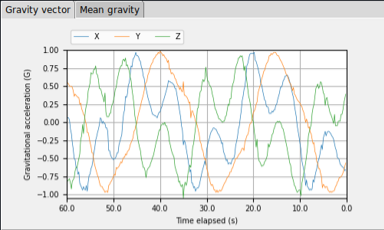
\includegraphics[scale=1.7]{grav_surowe}
		\caption{Dane z akcelerometru.}
		\label{fig:grav_raw}
	\end{subfigure}
	\hfill%
	\begin{subfigure}[h]{.49\textwidth}
		\centering
		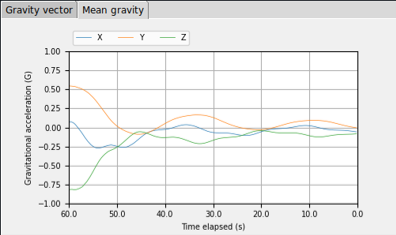
\includegraphics[scale=1.7]{grav_sr}
		\caption{Uśrednione wartości grawitacji.} 
		\label{fig:grav_mean}
	\end{subfigure}
	
	\caption{Przykładowe wykresy. Źródło: [opracowanie własne]}
	\label{fig:wykresy_gui}
	
\end{figure}

\section{Drzewo projektu}

Aplikacja napisana jest w konwencji obiektowej. Aby zachować zorganizowaną strukturę kodu źródłowego podzielony został on na wiele plików, w których znajdują się definicje klas o podobnych cechach lub działaniu. Rozdział ten służy przedstawieniu struktury aplikacji oraz krótkiemu opisowi, funkcji jakie pełni każdy z plików. Drzewo programu widoczne jest na Rys. \ref{fig:drzewo}. Plikiem uruchomieniowym jest plik \textbf{main.py}, który zawiera definicję klasy samej aplikacji oraz klasę menedżera interfejsu, odpowiedzialnego za zmiany aktywności jego elementów. Poszczególne moduły aplikacji odnoszą się do interfejsu właśnie przez ten obiekt, co znacznie poprawia czytelność oraz organizację kodu. W folderze \textit{config} znajduje się plik konfiguracyjny \textbf{config.yaml}, który zawiera adres oraz port na których postawiony ma zostać serwer TCP. Folder \textit{modules} zawiera kolejne katalogi \textit{backend}, \textit{gui} oraz \textit{properties}. W katalogu \textit{backend} umieszczono wszystkie pliki zawierające obiekty sterujące lub tworzące mechanizmy aplikacji, które nie są widoczne dla użytkownika. Zawierają się w tym pliki \textbf{clinostat\_com.py} zawierający moduł komunikacyjny klinostatu, \textbf{custom\_thread.py} w którym znajduje się zmodyfikowana klasa wątku oraz plik \textbf{data\_socket.py}, który zawiera definicję obiektu serwera TCP. Katalog \textit{gui} zawiera pliki związane z elementami interfejsu graficznego, na które składają się \textbf{segments.py} zawierający definicje poszczególnych modułów interfejsu oraz plik \textbf{custom\_tk\_widgets.py}, który zawiera pojedyncze, zmodyfikowane elementy interfejsu stworzone na potrzeby aplikacji. W ostatnim folderze \textit{properties} znajduje się plik \textbf{properties.py}, który zawiera specjalnie przygotowane struktury danych, przechowywujące zmienne, flagi oraz obiekty kluczowe dla działania aplikacji.

\begin{figure}[h]
	
	\centering
	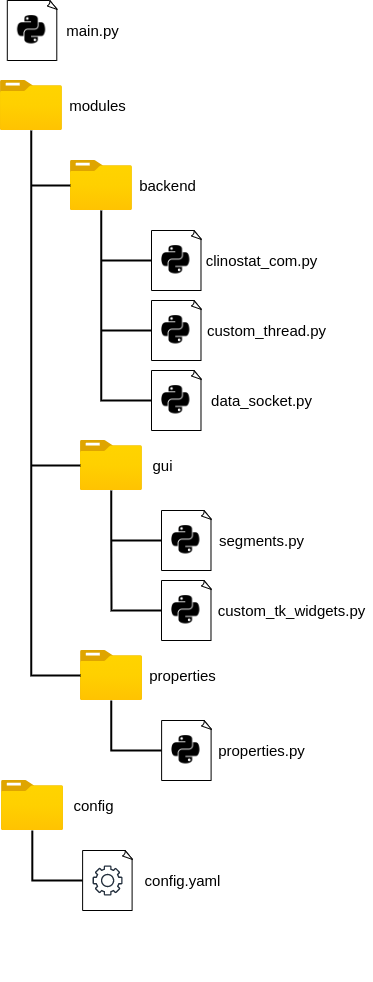
\includegraphics[scale=.34]{tree}
	\caption{Struktura plików aplikacji. Źródło: [opracowanie własne]} 
	\label{fig:drzewo}
	
\end{figure}
\section{Zabezpieczenia aplikacji}

Po wstępnym ukończeniu aplikacji poddano ją szczegółowym testom, przeprowadzanym przez kilka niezwiązanych z nią wcześniej osób. Miało to na celu wykrycie ukrytych błędów, przetestowanie jak największej ilości kombinacji wysłanych komend, zbadanie reakcji aplikacji na nadużycie dostępnych operacji oraz innych niepożądanych efektów, których wystąpienie nie zostało przewidziane na etapie jej tworzenia. Testy te pozwoliły na stworzenie zabezpieczeń uniemożliwiających operatorowi urządzenia wykonania niedozwolonych operacji oraz wykrywających konflikty powstałych na drodze interakcji operacji użytkownika oraz zachodzących w tle zautomatyzowanych procesów. Najprostszym zabezpieczeniem obecnym w aplikacji jest tymczasowa dezaktywacja interfejsu odpowiedzialnego za komendy wysyłane przez port szeregowy. Jeśli wysłana komenda powoduje wysłane odpowiedzi ze strony kontrolera klinostatu, to część elementów interfejsu zostaje dezaktywowana do czasu jej otrzymania, lub do maksymalnego czasu oczekiwania. Zapobiega to wysłaniu przez użytkownika komendy w momencie gdy do klinostatu przekazywane są przykładowo bajty określające prędkość obrotów. Aplikacja posiada również zautomatyzowany system wysyłania komendy nawadniania w momencie kiedy minął odpowiedni czas. Stwarza to możliwość próby wysłania takiej komendy podczas np. oczekiwania na odpowiedź ze strony klinostatu. Brak zabezpieczeń spowodowałby uzyskanie nieprawidłowej odpowiedzi z urządzenia co doprowadziłoby do błędu. Problem ten rozwiązano tworząc obiekt specjalnego wątku, który wykorzustuje strukturę synchronizacyjną \textbf{lock} aby uniemożliwić dostęp innym wątkom do portu szeregowego podczas oczekiwania na komendę. Po zakończeniu pracy wątek odblokowywuje port szeregowy i zakolejkowana instrukcja zostaje wysłana. Klinostat może zostać również fizycznie odłączony od komputera podczas pracy. Aplikację oraz urządzenie chronią tutaj dwa mechanizmy. Pierwszy z nich wynika z samej konstrukcji elektroniki klinostatu, która wymaga połączenia z komputerem przez port USB aby uzyskać zasilanie sekcji logicznej. Zerwanie połączenia automatycznie spowoduje odcięcie zasilania kontrolera i zatrzymanie klinostatu. Natomiast wysłanie komendy do odłączonego portu wygeneruje błąd w aplikacji, co skutkuje jej zawieszeniem. Rozwiązaniem tego problemu było stworzenie specjalnej metody \textbf{device\_likely\_unplugged} klasy aplikacji, która wykonywana jest przez wątek obsługujący port szeregowy w momencie zgłoszenia przez niego wyjątku (ang. \angver{exception}). Wykonanie tej metody powoduje całkowite zresetowanie aplikacji i wyświetlenie stosownego komunikatu o błędzie, sugerującego sprawdzenie połączenia przewodu USB.
\begin{lstlisting}[language=Python,caption={Metoda wykrywająca odłączone urządzenie.}]
def device_likely_unplugged(self) -> None:

	try:
		self.params["device"].close_serial()
		
	except clinostat_com.ClinostatCommunicationError:
		pass
		
	self.params["device"] = None
	self.interface_manager.ui_modes_reset()
	self.flags["pumping"] = False
	self.trackers = properties.AppTrackers()
\end{lstlisting}